%----------------------------------------------------------------------------------------
\chapter{Design}
\label{chap:design}
%----------------------------------------------------------------------------------------

This chapter outlines the architectural design of the Kotlin DSL for Alchemist. 
The proposed solution aims to reconcile the static type safety of the host language with the dynamic requirements of the simulator,
 specifically the need for arbitrary class loading and batch execution.

The design process focused on three key areas. 
\begin{itemize}
    \item \textbf{Component Instantiation}: the architecture shifts the responsibility of component instantiation 
    from the framework's reflection mechanism to the language itself, allowing for direct usage of Alchemist APIs.
    \item \textbf{Context System}: a hierarchical context system is introduced to enforce domain rules and structural correctness at compile time, mirroring the containment logic of the simulation model.
    \item \textbf{Deferred Execution}: a deferred execution strategy is employed to support parametric simulations, ensuring that a single script definition can generate multiple independent simulation instances.
\end{itemize}

\newpage

\section{Design Foundations}

The architectural strategy exploits the capabilities of Kotlin as a General-Purpose Language (GPL)
 to achieve seamless integration with the existing Alchemist ecosystem.
The main design decision is to grant users direct access to the underlying Alchemist codebase,
allowing users to instantiate these classes directly using standard Kotlin syntax, 
leveraging the fact that Alchemist components are native Java or Kotlin objects.

This approach eliminates the need for reflective class loading as described in \Cref{sec:loadingphase2}, 
shifting the responsibility 
of object instantiation from the framework to the language itself.
For instance, instantiating a \textit{network model} component becomes a direct constructor call:

\begin{minted}[fontsize=\footnotesize, linenos]{kotlin}
val networkModel = ConnectWithinDistance(0.5)
\end{minted}

In contrast, the YAML equivalent requires an indirect specification:
\begin{minted}[fontsize=\footnotesize, linenos]{yaml}
network-model:
  type: ConnectWithinDistance
  parameters: [0.5]
\end{minted}

By exposing the underlying API directly, the DSL inherits the type safety and tooling support of the host language. 
Users are compelled by the compiler to provide correct argument types and counts,
transforming what were previously runtime configuration errors into compile-time checks.
Furthermore, this design ensures immediate compatibility with any future extensions to the Alchemist core,
as any new class on the \textit{classpath} is automatically available for use within the DSL 
without requiring updates to the parser logic.

Given this design decision, the next sections will detail how the new system should
 integrate with the existing loading system of Alchemist, 
and describe the design decisions made for the DSL itself.

\subsection{Loading System Integration}

To integrate with the existing Alchemist loading system, 
the proposed architecture introduces a new implementation of the \textbf{Loader} interface. 
As established in \Cref{sec:loadingphase1}, the \texttt{Loader} serves as a factory for simulation instances, 
parameterized by a set of variables that must be used in that specific simulation instance. 
The core mechanism relies on the method:

\begin{minted}[fontsize=\footnotesize, linenos, ignorelexererrors = true]{kotlin}
fun <T, P : Position<P>> getWith(values: Map<String, *>): Simulation<T, P>
\end{minted}

It \textbf{instantiates} a simulation by mapping variable names to the given set of specific values. 
This design decouples the generation of the simulation model from the management of configuration variables, 
allowing a single \texttt{Loader} to generate multiple simulation instances with distinct parameter sets, 
an important enabler for batch execution.

The execution lifecycle is instead managed by the \texttt{Launcher} interface,
which accepts a \texttt{Loader} as a dependency. 
The \texttt{Launcher} is responsible for identifying the \textbf{variable space} (e.g., iterating over a set of parameters) 
and invoking the \texttt{Loader} \texttt{getWith(values: Map<String, \*>)} method to create 
the corresponding simulation instances. 

\begin{figure}
    \centering
    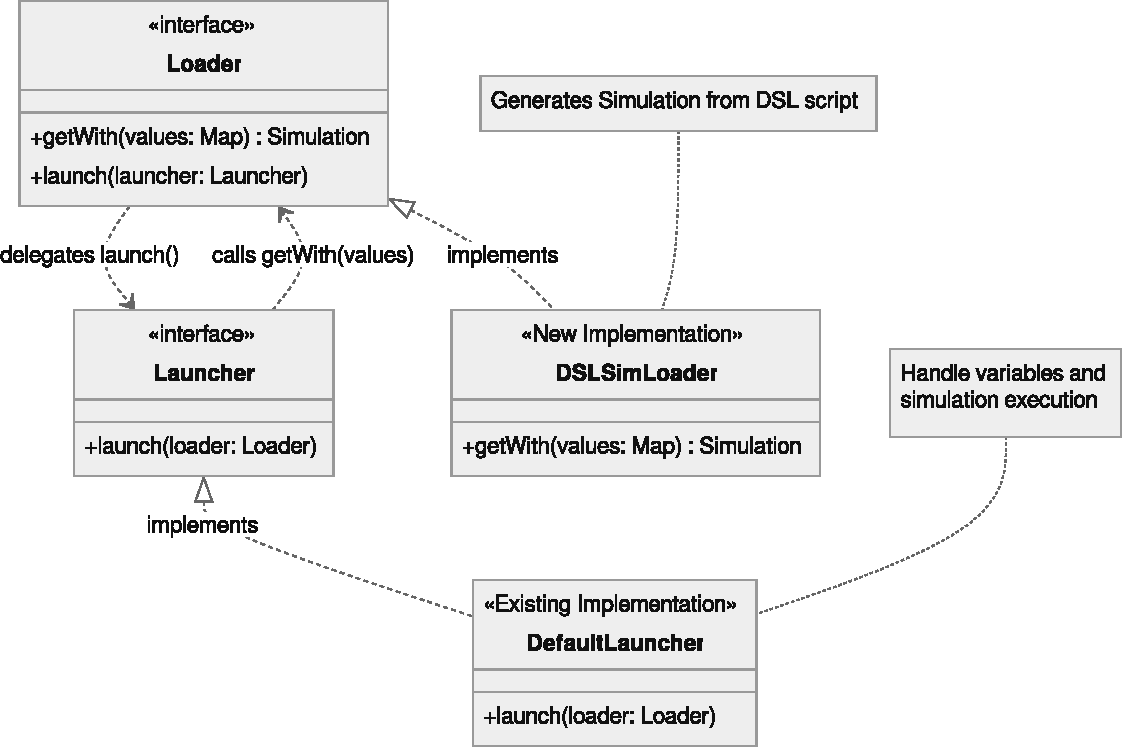
\includegraphics[width=\textwidth]{figures/launcherloader.pdf}
    \caption{Loading system architecture showing the bidirectional 
    relationship between the Launcher and Loader components.}
    \label{fig:launcherLoader}
\end{figure}

As shown in \Cref{fig:launcherLoader}, the relationship between these components exhibits a bidirectional binding:
\begin{itemize}
    \item The \texttt{Launcher} depends on the \texttt{Loader} to obtain the simulation instance 
    (via the \texttt{getWith(values: Map<String, *>)} method).
    \item The \texttt{Loader} holds a reference to the specified \texttt{Launcher}, since the loader is the component 
    that holds all information needed to generate a simulation given the user configuration. The \texttt{Launcher} is a 
    configurable component that can be specified by the user to control the execution of the simulation.
\end{itemize}


The loader component is the one that should actually be used to launch the simulation, using its 
\texttt{launch()} method.

By adhering to this established contract, 
the new DSL-based implementation achieves full interoperability with the existing ecosystem. 
It acts as an alternative to the legacy loader, 
allowing existing \texttt{Launcher} implementations to use the new DSL-based loader transparently 
via the \textit{Inversion of Control} (IoC) pattern.
Consequently, the complexity of the loading mechanism remains hidden from the user,
who retains the flexibility to specify custom \emph{Launchers} without coupling the loader instance 
to a specific underlying \texttt{Loader} implementation.


\subsection{Scoped Information Contexts}

To maintain the same semantics as the YAML configuration file and enforce domain rules, 
the architecture employs a \textit{Scoped Information Context} pattern. 
The simulation configuration is modeled not as a flat list of properties, but as a 
hierarchy of \textbf{nested contexts}, 
mirroring the structural containment of the domain entities.

In this model, the availability of operations and data is strictly determined by the current scope. 
For instance, the definition of a reaction makes sense only within the context of a node or a global program.
This design mimics the nesting levels in the YAML configuration file, but in a more \textit{type-safe} way.
While the YAML file allows, for example, defining a \textit{Deployment} inside a \textit{Deployment}, the nested context 
prevents the user from defining such a configuration, since at each context level, only the allowed operations and data are available.
The relationship between the components, as shown in \Cref{fig:scoped-contexts}, is the following:

\begin{itemize}
    \item \textbf{Simulation Context} is the root context; it contains all the execution settings, 
    as described in \Cref{sec:execution-settings}; 
    \item \textbf{Deployments Context} handles the creation of node deployments;
    \item \textbf{Deployment Context} configures a specific deployment instance;
    \item \textbf{Content Context} defines the molecules and concentrations for nodes;
    \item \textbf{Programs Context} manages the reaction programs for nodes;
    \item \textbf{Program Context} specifies the details of a reaction;
    \item \textbf{Properties Context} manages node properties;
    \item \textbf{Property Context} assigns properties to nodes;
    \item \textbf{Exporter Context} configures data export;
    \item \textbf{Layer Context} defines spatial layers;
    \item \textbf{Terminators Context}, \textbf{Output Monitors Context}, 
    and \textbf{Global Programs Context} allow the addition of respective components.
\end{itemize}

This hierarchical design has been extracted from the Alchemist YAML specification 
and represents a direct translation of the YAML hierarchy into the DSL, with some minor syntax 
changes.

\begin{figure}
    \centering
    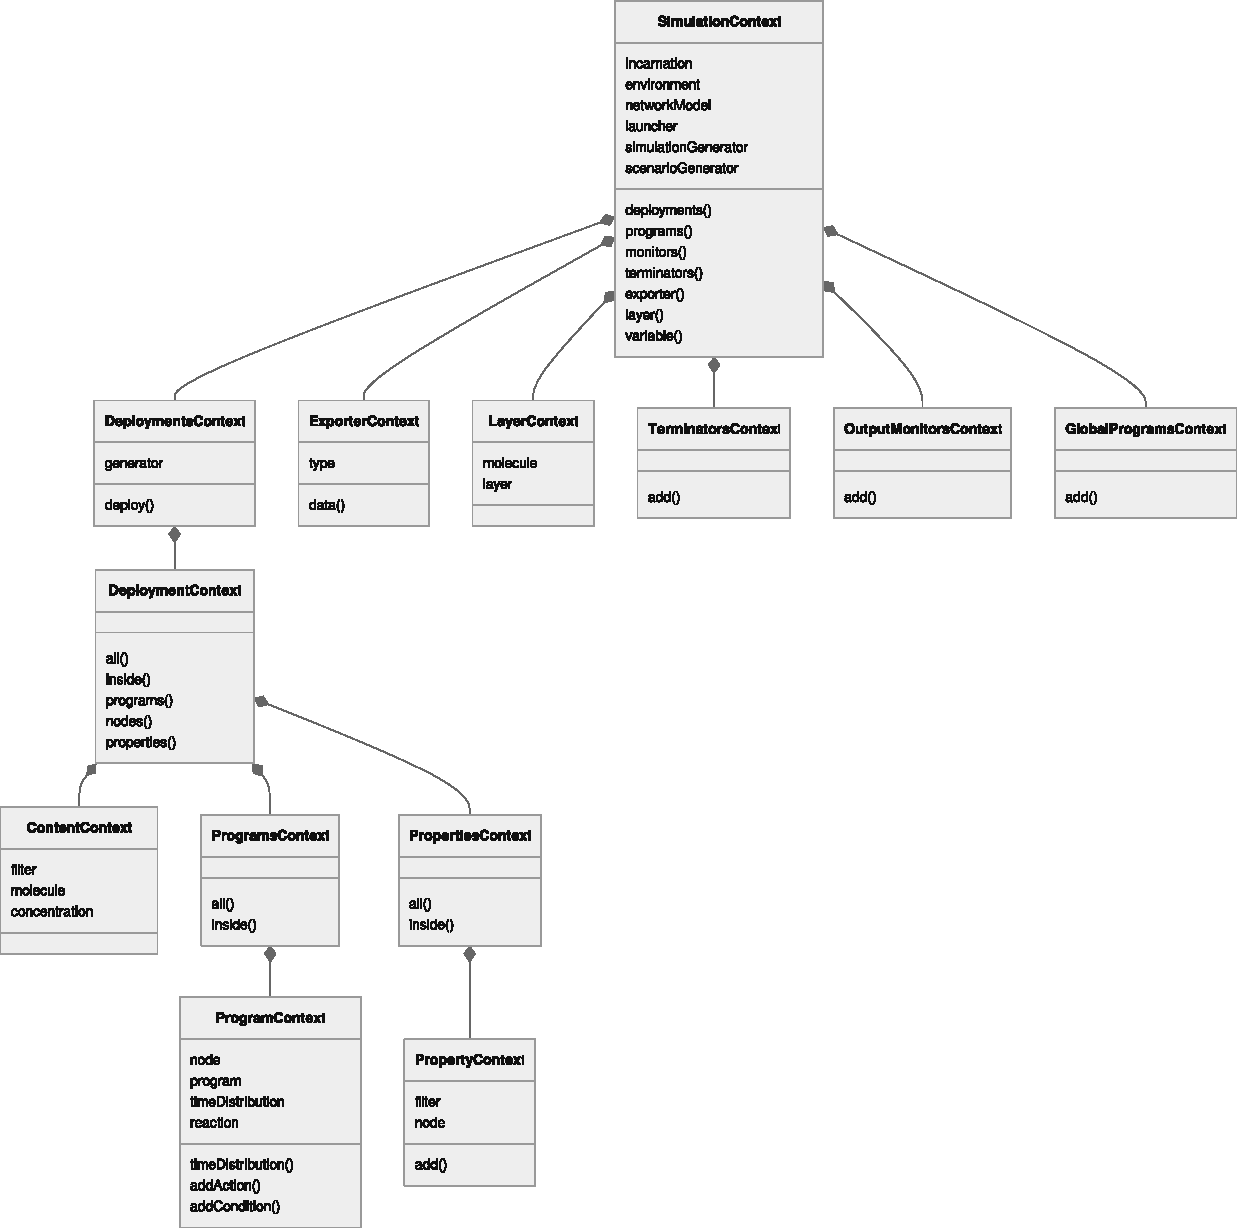
\includegraphics[width=\textwidth]{figures/contexts.pdf}
    \caption{Hierarchical structure of Scoped Information Contexts in the DSL, 
    illustrating the nested containment relationships.}\label{fig:scoped-contexts}
\end{figure}

This hierarchical design serves two purposes:
\begin{enumerate}
    \item \textbf{Scope Containment}: it prevents structural inconsistencies by restricting the visibility of methods.
     A user cannot accidentally define a deployment inside a deployment because the \textit{Deployment Context} 
     does not expose the API for deployment creation.
    \item \textbf{Context Awareness}: inner scopes transparently inherit relevant information from outer scopes. 
    A node definition context automatically has access to the environment type defined in the parent scope, 
    eliminating the need for redundant type specifications.
\end{enumerate}

\section{Detailed Design}

This section details the design choices and mechanisms that enable the DSL to function as a flexible configuration template,
 capable of supporting multiple simulation runs with varying parameters. 

To achieve this goal, the design addresses two fundamental challenges:
\begin{itemize}
    \item \textbf{Deferred Execution}: preventing immediate instantiation of simulation components to allow for parametric configuration across batch runs.
    \item \textbf{Variable Management}: abstracting variables from direct values to contextual references, ensuring that the same script can be re-evaluated with different parameter sets.
\end{itemize}

\subsection{Deferred Execution Model}

A critical requirement for the Alchemist simulator is the support for \textit{batch executions}, 
where a single configuration file generates multiple simulation instances with varying parameters. 
A naive implementation of the DSL might instantiate the simulation objects immediately during script execution. 
However, this would bind the simulation to a single set of values, breaking the batching requirement.

To address this, the design adopts a \textbf{Lazy Evaluation} model, essentially a variation of the 
\textit{Command Pattern}\footnote{\url{https://archive.is/vwOm2}}. 
When the DSL script is executed, it does not construct the simulation entities (nodes, deployments, reactions) directly. 
Instead, it records a sequence of \emph{build tasks} or specifications. 
This already happens in the current YAML loader, 
where the simulation model is actually built only when the \texttt{getWith()} method of the loader is invoked.


The process is divided into two distinct phases:
\begin{enumerate}
    \item \textbf{Definition Phase}: The script runs once. 
    It builds an internal representation of the user's intent, a recipe for how to build the simulation. 
    Each DSL operation is stored as a \textbf{build step}, which will later be executed to modify the simulation model.
    During this phase, variables are treated as symbolic references rather than concrete values. 
    Variables must not be accessed during this phase, since they are not yet assigned any value. This phase should produce 
    a \texttt{SimulationContext} instance that stores all the needed information to 
    later allow the DSL loader component to materialize the simulation model, 
    given the variable values for the current run. This \texttt{SimulationContext} instance should be considered the \textit{recipe}
    of the simulation, which will later be used to materialize the simulation model.
    \item \textbf{Materialization Phase}: This occurs repeatedly, once for each simulation in a batch. 
    The \textit{DSL Loader} invokes the recorded build tasks of the given \texttt{SimulationContext} instance 
    after injecting the specific variable values (the \textit{grounding}) 
    for the current run.
\end{enumerate}

\begin{figure}
    \centering
    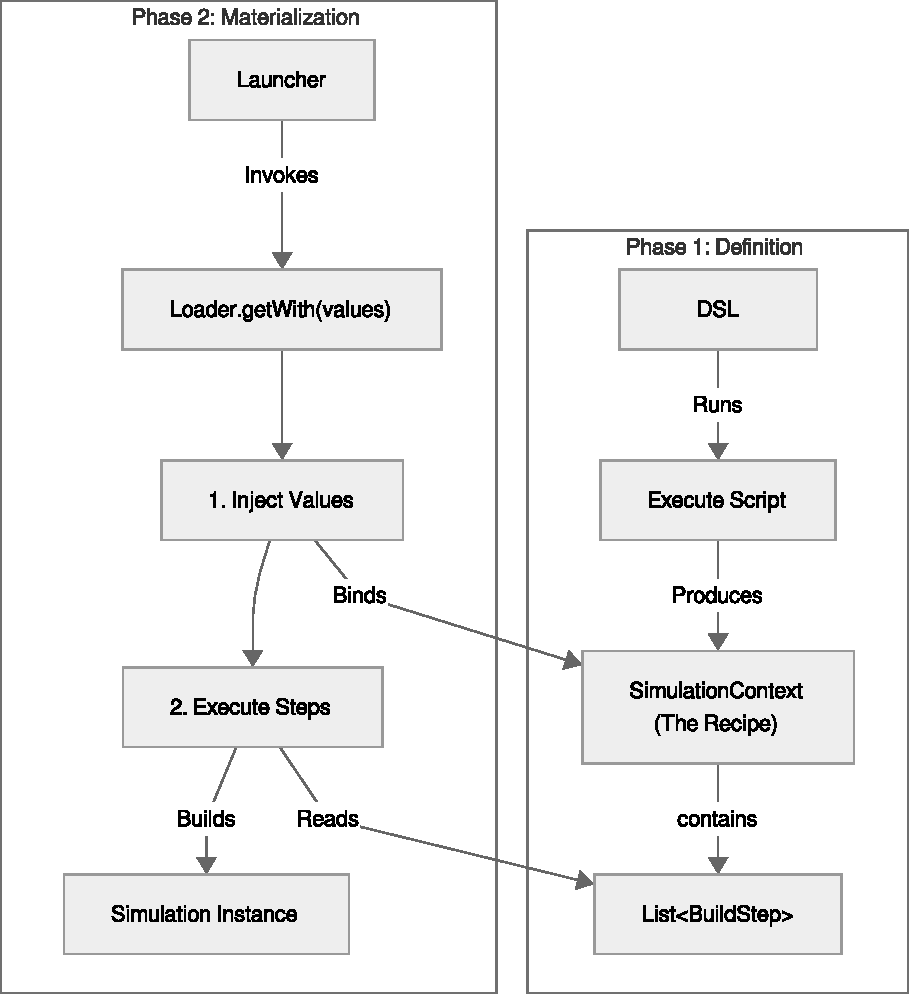
\includegraphics[width=0.7\textwidth]{figures/lazyeval.pdf}
    \caption{Lazy Evaluation model diagram illustrating the two-phase execution strategy,
    the Definition Phase and the Materialization Phase.}\label{fig:lazyeval}
\end{figure}


Since the user should be able to reference variables in the DSL, the lazy evaluation design prevents
the DSL execution from accessing variable values that are not yet assigned by the launcher. If the DSL 
script were directly executed during its evaluation phase, the variables would be accessed before they are assigned
any values. Moreover, directly executing the DSL script would require re-executing 
the script for each simulation in the batch. 


This separation of concerns ensures that the computational overhead of evaluating the script is paid only once,
 while the lightweight \emph{materialization phase} can be repeated efficiently for a batch of independent runs.

\subsection{Variables Management}

One of the primary challenges in adapting a General-Purpose Language for simulation configuration is the handling
of variable state across batch executions.
In a standard imperative program, variable assignment is immediate and bound to the current execution scope.
However, the Alchemist batch execution model requires the same configuration logic to be re-evaluated against 
a changing set of parameters. 
If variables were resolved at the time of script definition, 
the simulation would be bound to a single static configuration, negating the purpose of the batch mechanism.

To address this, the proposed design abstracts the concept of a variable from a direct value holder 
to a \textbf{reference} to a certain value in a \textbf{variable registry}. 
Leveraging the semantic capabilities of the host language, 
variables defined in the DSL do not store data directly. 
Instead, they function as keys that query a centralized \texttt{VariablesContext}, a scoped container responsible
for managing the state of the simulation parameters.

Under this paradigm, the declaration of a variable registers the identifier within
 the context but defers value resolution. 
 The actual binding of values occurs solely during the \textit{materialization phase} described in the previous section. 
 When the \texttt{Loader} prepares a specific simulation instance, 
 it populates the \texttt{VariablesContext} with the distinct combination of parameters assigned to that run.
Consequently, when the DSL logic subsequently accesses the variable, the request is fetched from the \texttt{VariablesContext}.

This architecture effectively decouples the definition of the simulation structure from the data that drives it.
It ensures that the same compilation of the DSL script can support an arbitrary number of execution instances,
 each perceiving a unique, consistent view of the variable space. 
\Cref{fig:variable-proxy} shows this interaction.

\begin{figure}
    \centering
    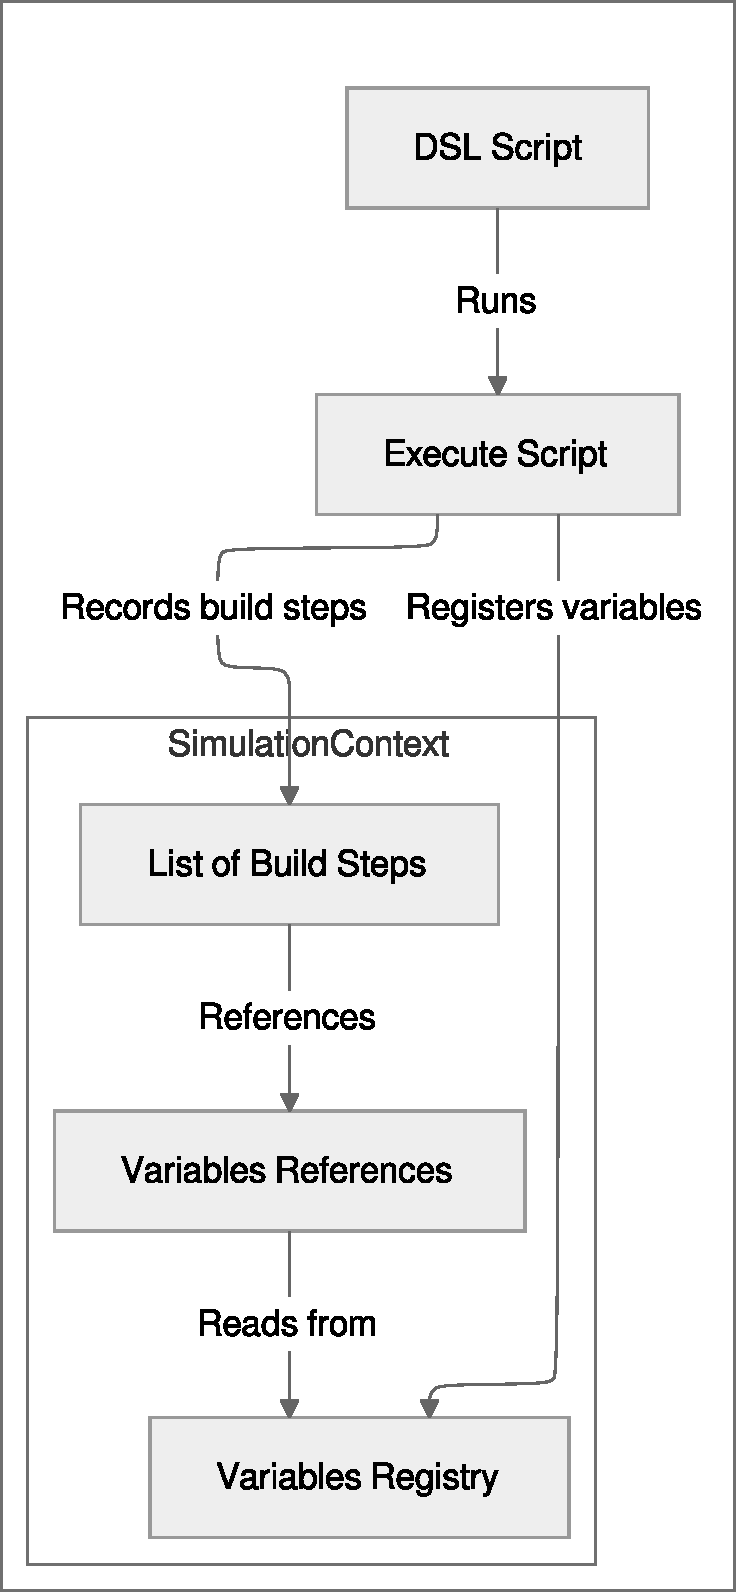
\includegraphics[width=0.53\textwidth]{figures/variablesdesign.pdf}
    \caption{Variables Context design diagram illustrating how variables 
    function as references to a centralized variable registry rather than direct value holders.}
    \label{fig:variable-proxy}
\end{figure}

The low-level details of this mechanism,
particularly the integration with Kotlin language features, are provided in the Implementation chapter.
